\documentclass[svgnames,11pt]{beamer}
\input{/home/tof/Documents/Cozy/latex-include/preambule_commun.tex}
\input{/home/tof/Documents/Cozy/latex-include/preambule_beamer.tex}
\usepackage{pgfpages} \setbeameroption{show notes on second screen=left}
\author[]{Christophe Viroulaud}
\title{Outils numériques}
\date{\framebox{\textbf{Web 01}}}
%\logo{}
\institute{Seconde - SNT}

\begin{document}
\begin{frame}
\titlepage
    \note[item]{\fcolorbox{black}{red}{{\LARGE Partie 1 au tableau}}}
    \note[item]{\fcolorbox{black}{red}{{\LARGE Créer une \emph{information Pronote}}}: la phrase cachée est \emph{vive l'informatique}}
    \note[item]{\fcolorbox{black}{red}{{\LARGE Publier l'évaluation \emph{lycée connecté}}}: entraînement rentrée}
    \note[item]{\fcolorbox{black}{red}{{\LARGE Mettre entrainement\_dossier.zip sur site}}}
\end{frame}
\begin{frame}
    \frametitle{}

En plus des cours en présentiel, il est possible d'interagir avec l'équipe enseignante de plusieurs manières.

\vspace{2cm}
\framebox{Quels sont les outils numériques proposés dans l'établissement?}

\end{frame}
\section{Site SNT}
\begin{frame}
    \frametitle{Site SNT}

\begin{activite}
\begin{enumerate}
    \item Se rendre sur le site web:
    \begin{center}
        {\Large \url{https://cviroulaud.github.io}}
    \end{center}
    \item Cliquer sur le bouton \textbf{\texttt{Voir les cours}} de la section \emph{seconde}.
    \item Ouvrir le slide \textbf{\texttt{Outils numériques}}.
\end{enumerate}
\end{activite}
\begin{center}
\centering
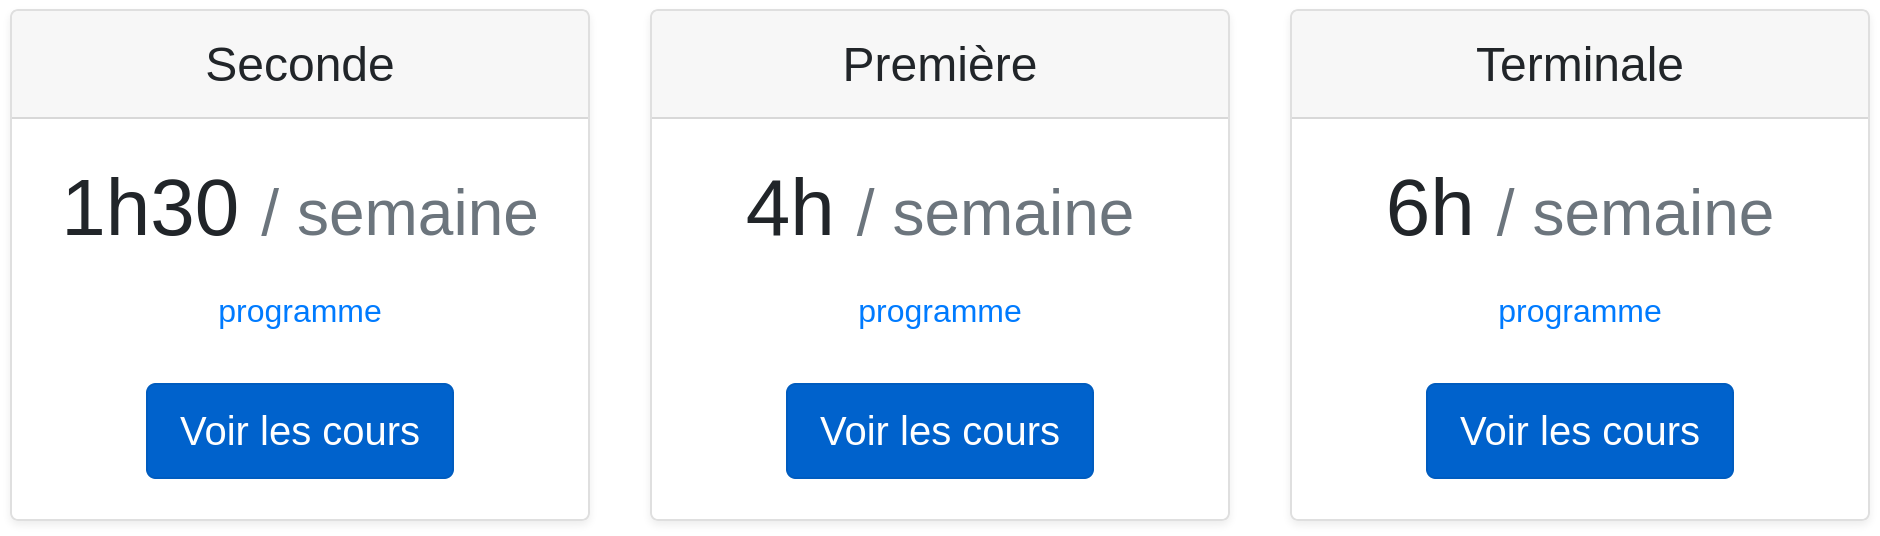
\includegraphics[width=9cm]{ressources/site.png}
\captionof{figure}{Site SNT / NSI} 
\label{IMG}
\end{center}
\end{frame}
\section{Pronote}
\begin{frame}
    \frametitle{Pronote}

Chaque élève possède un accès \emph{Pronote} grâce à l'identifiant fourni en début d'année.

\end{frame}
\begin{frame}
    \frametitle{}

    Il est possible d'accéder à Pronote via son smartphone:
    \begin{itemize}
        \item \href{https://play.google.com/store/apps/details?id=com.IndexEducation.Pronote&hl=fr&gl=US}{Google Play}
        \item \href{https://apps.apple.com/fr/app/pronote/id1138223804}{App Store}
    \end{itemize}
\begin{center}
\centering
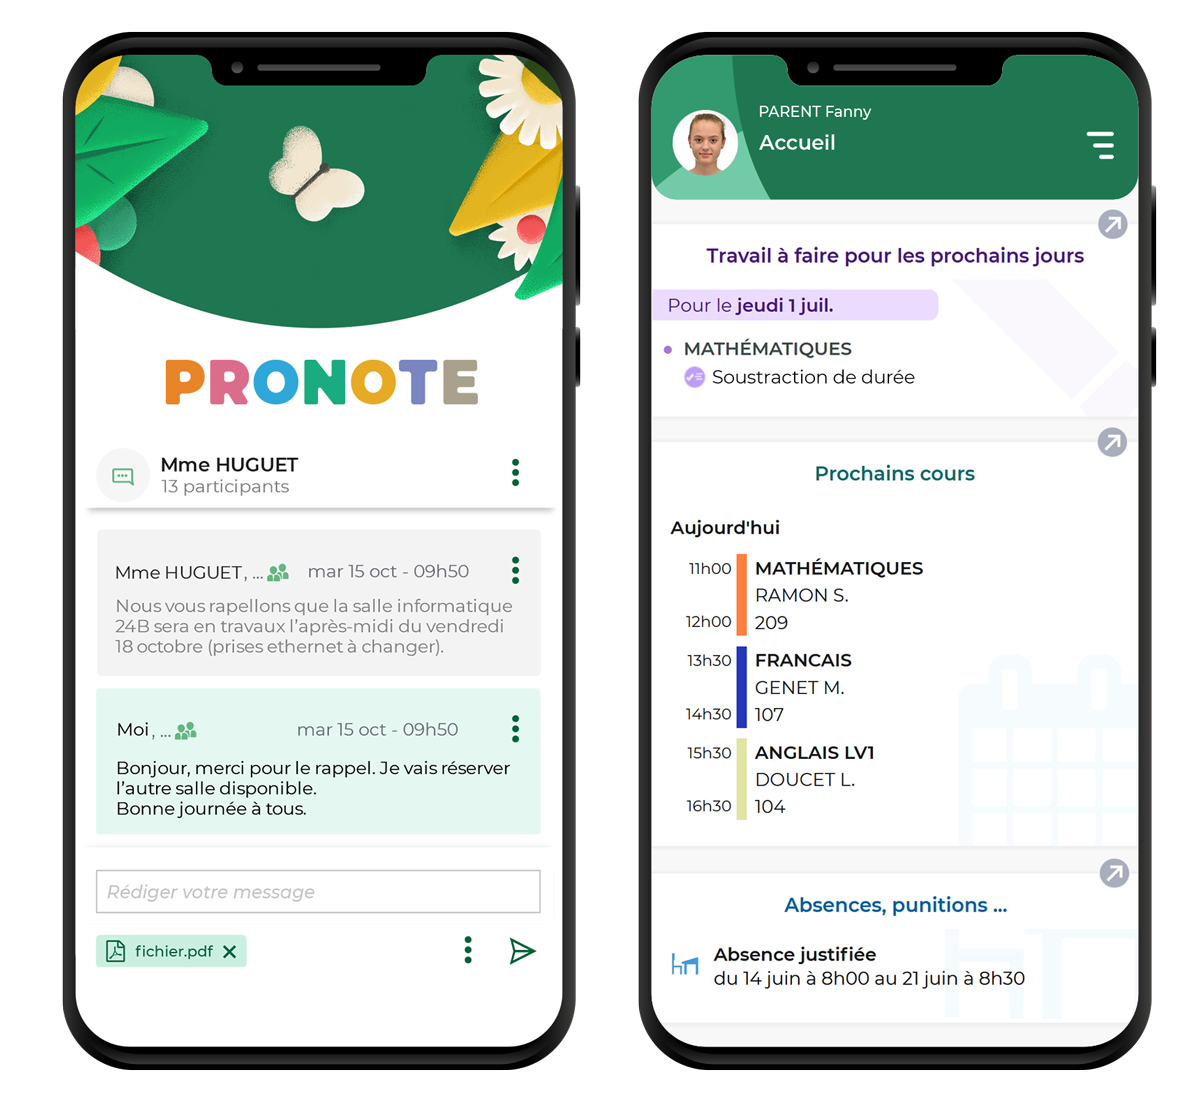
\includegraphics[width=5cm]{ressources/screen-pronote-2021.png}
\captionof{figure}{Rendu de l'application}
\label{IMG}
\end{center}
\end{frame}
\begin{frame}
    \frametitle{}

Il est également possible d'accéder au site web de Pronote. Un lien est disponible en haut à droite du site de \emph{Jay de Beaufort}.
\begin{center}
    {\Large         \url{https://lyceejaydebeaufort.fr/}
    }
\end{center}
\begin{center}
    
\includegraphics[width=1cm]{ressources/pronote.png}
\end{center}
\end{frame}
\begin{frame}
    \frametitle{}

    \begin{activite}
    \begin{enumerate}
        \item Se rendre sur le site de Pronote et se connecter.
        \item Dans l'onglet \emph{Communication}, ouvrir une \emph{discussion} avec le professeur.
        \item Dans \emph{Informations et sondages} découvrir la phrase cachée. Marquer le message comme \emph{lu}.
    \end{enumerate}
    \end{activite}
\begin{aretenir}[]
Ces deux onglets sont des moyens de communication très utilisés dans l'établissement. Il faut impérativement savoir les utiliser.
\end{aretenir}
\end{frame}
\section{Lycée connecté}
\begin{frame}
    \frametitle{Lycée connecté}

    Le \emph{lycée connecté} est un outil très complet. Il propose de nombreux outils comparables à ceux d'un compte Google auxquels s'ajoutent des applications orientées éducation.

\end{frame}
\subsection{Connexion}
\begin{frame}
    \frametitle{Connexion}

    Pour accéder au \emph{lycée connecté} un lien est disponible en haut à droite du site de \emph{Jay de Beaufort}.
\begin{center}
    {\Large         \url{https://lyceejaydebeaufort.fr/}
    }
\end{center}
\begin{center}
    
\includegraphics[width=1cm]{ressources/ent.jpg}
\end{center}

\end{frame}
\begin{frame}
    \frametitle{}

    \begin{activite}
    \begin{enumerate}
        \item Se rendre sur la page web du \emph{lycée connecté}.
        \item Cliquer sur \textbf{se connecter}.
        \item Cliquer sur le lien \ref{eleve}.
        \begin{center}
        \centering
        
\includegraphics[width=8cm]{ressources/educonnect2021.png}
        \label{eleve}
        \end{center}
        \item Entrer les identifiants \emph{EduConnect} fournis.
        \item Penser à fournir un mail de récupération.
    \end{enumerate}
    \end{activite}

\end{frame}
\begin{frame}
    \frametitle{}

    La page d'accueil (figure \ref{accueil}) se découpe principalement en trois parties:
\begin{itemize}
\item le fil de nouveautés,
\item les widgets à gauche,
\item le bandeau de navigation en haut à droite.
\end{itemize}
\begin{center}
\centering
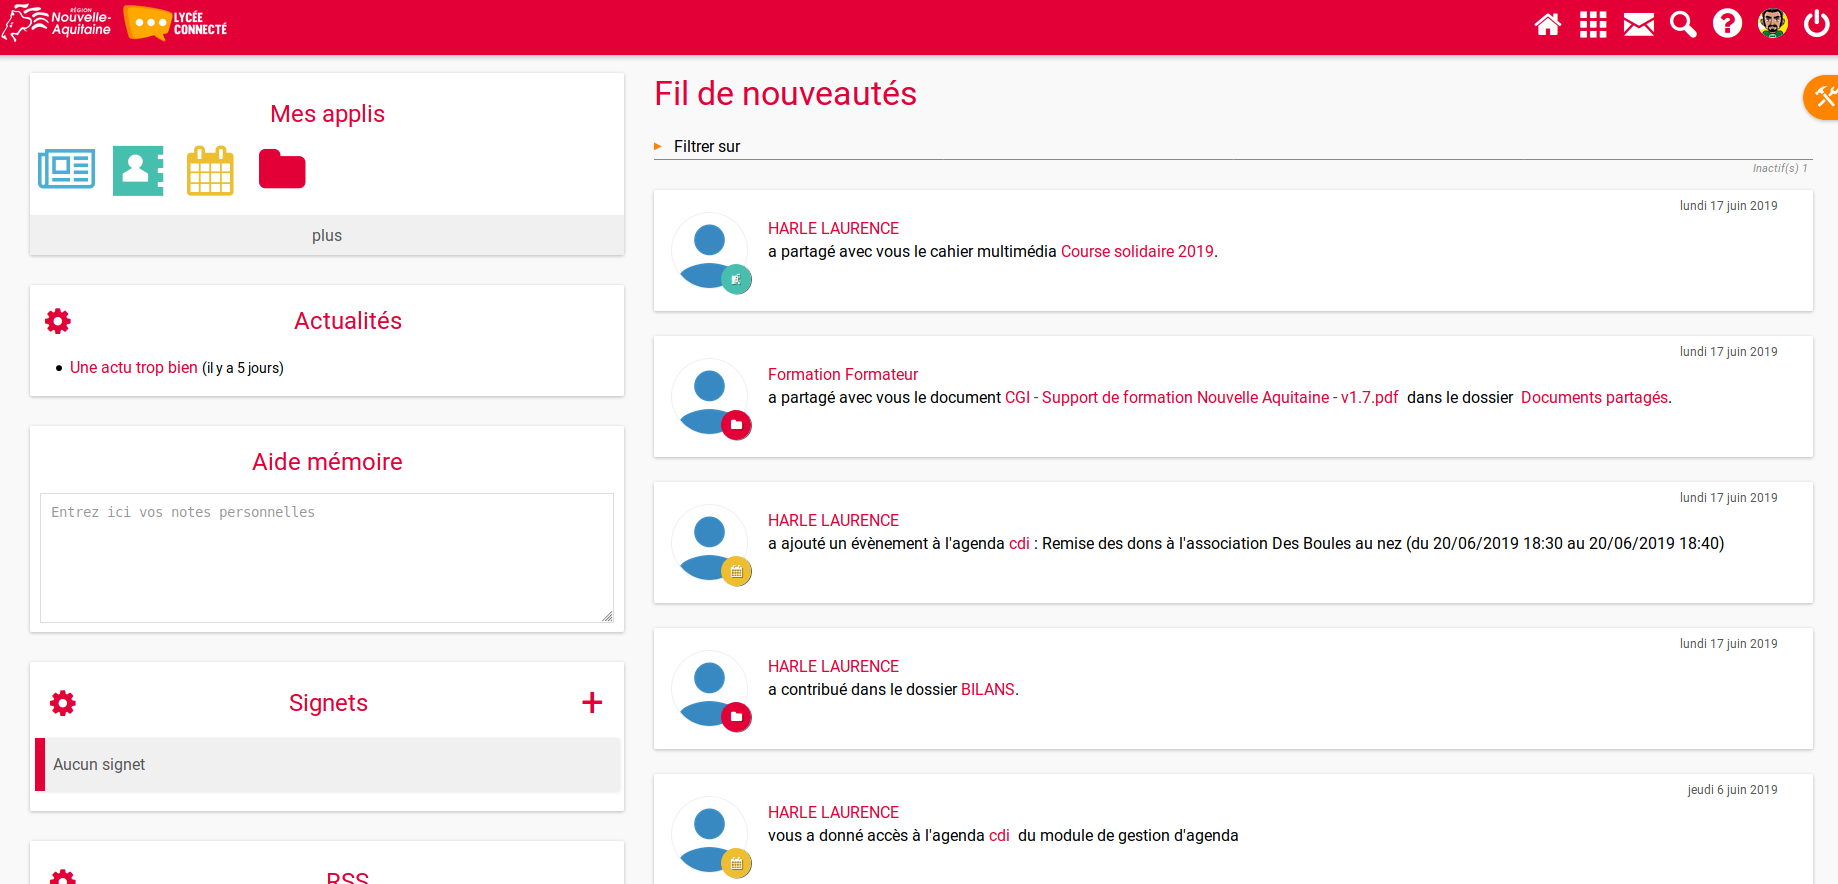
\includegraphics[width=8cm]{ressources/timeline.png}
\captionof{figure}{Page d'accueil}
\label{accueil}
\end{center}

\end{frame}
\subsection{Mail}
\begin{frame}
    \frametitle{}

    Chaque inscrit sur le \emph{lycée connecté} possède une adresse mail.
    \begin{activite}
    \begin{enumerate}
        \item Cliquer sur l'icône \textbf{Mon compte}:
        \begin{center}
        \centering
        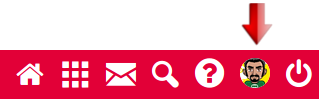
\includegraphics[width=5cm]{ressources/bandeaucompte.png}
        \end{center}
        \item Cliquer sur l'onglet \textbf{Messagerie}.
        \item Repérer l'adresse mail personnelle.
    \end{enumerate}
    \end{activite}

\begin{aretenir}[Remarque]
Il s'agit d'une véritable adresse mail similaire à gmail, hotmail, yahoo\dots Elle peut donc être utilisable pour communiquer avec des personnes extérieures au \emph{lycée connecté}.
\end{aretenir}

\end{frame}
\begin{frame}
    \frametitle{}

    \begin{activite}
    \begin{enumerate}
        \item Cliquer sur l'icône \textbf{Mail}:
        \begin{center}
        \centering
        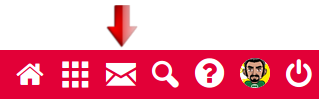
\includegraphics[width=5cm]{ressources/bandeauappmail.png}
        \end{center}
        \item Envoyer un nouveau message:
        \begin{center}
            \centering
            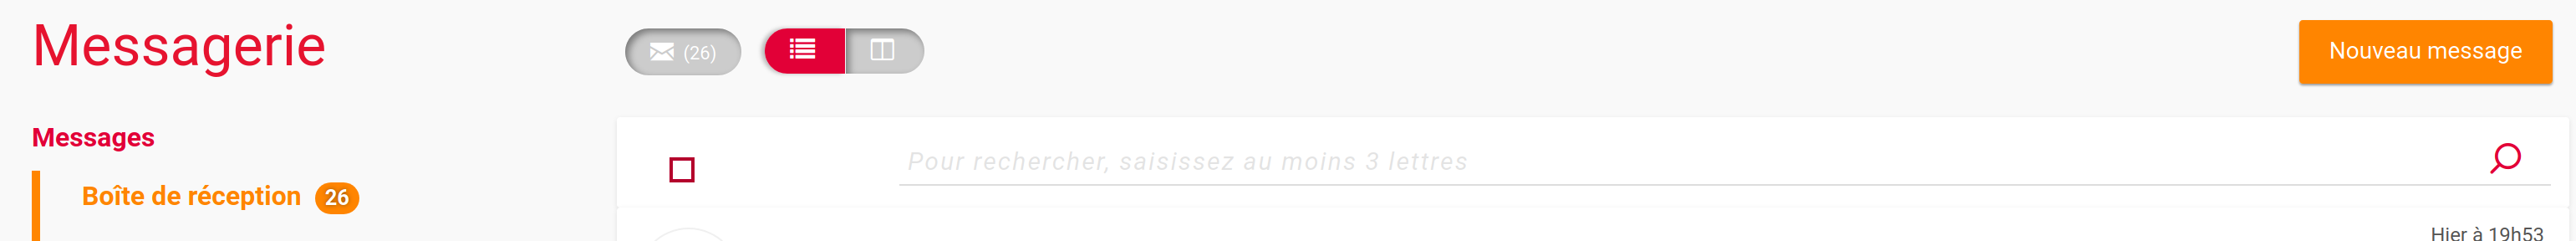
\includegraphics[width=9cm]{ressources/nouveaumessage.png}
            \end{center}

    \end{enumerate}

    \end{activite}
\begin{center}
    À suivre page suivante
\end{center}
\end{frame}
\begin{frame}
    \frametitle{}
    \setcounter{compteuractivite}{4}

    \begin{activite}
    \begin{enumerate}
        \setcounter{enumi}{2}
        \item Écrire un mail à \emph{Viroulaud Christophe}. Ce message décrira en quelques lignes les perspectives d'avenir (métier, projet d'orientation, spécialités envisagées pour la première). \\ Il faudra compléter les points suivants:
        \begin{center}
        \centering
        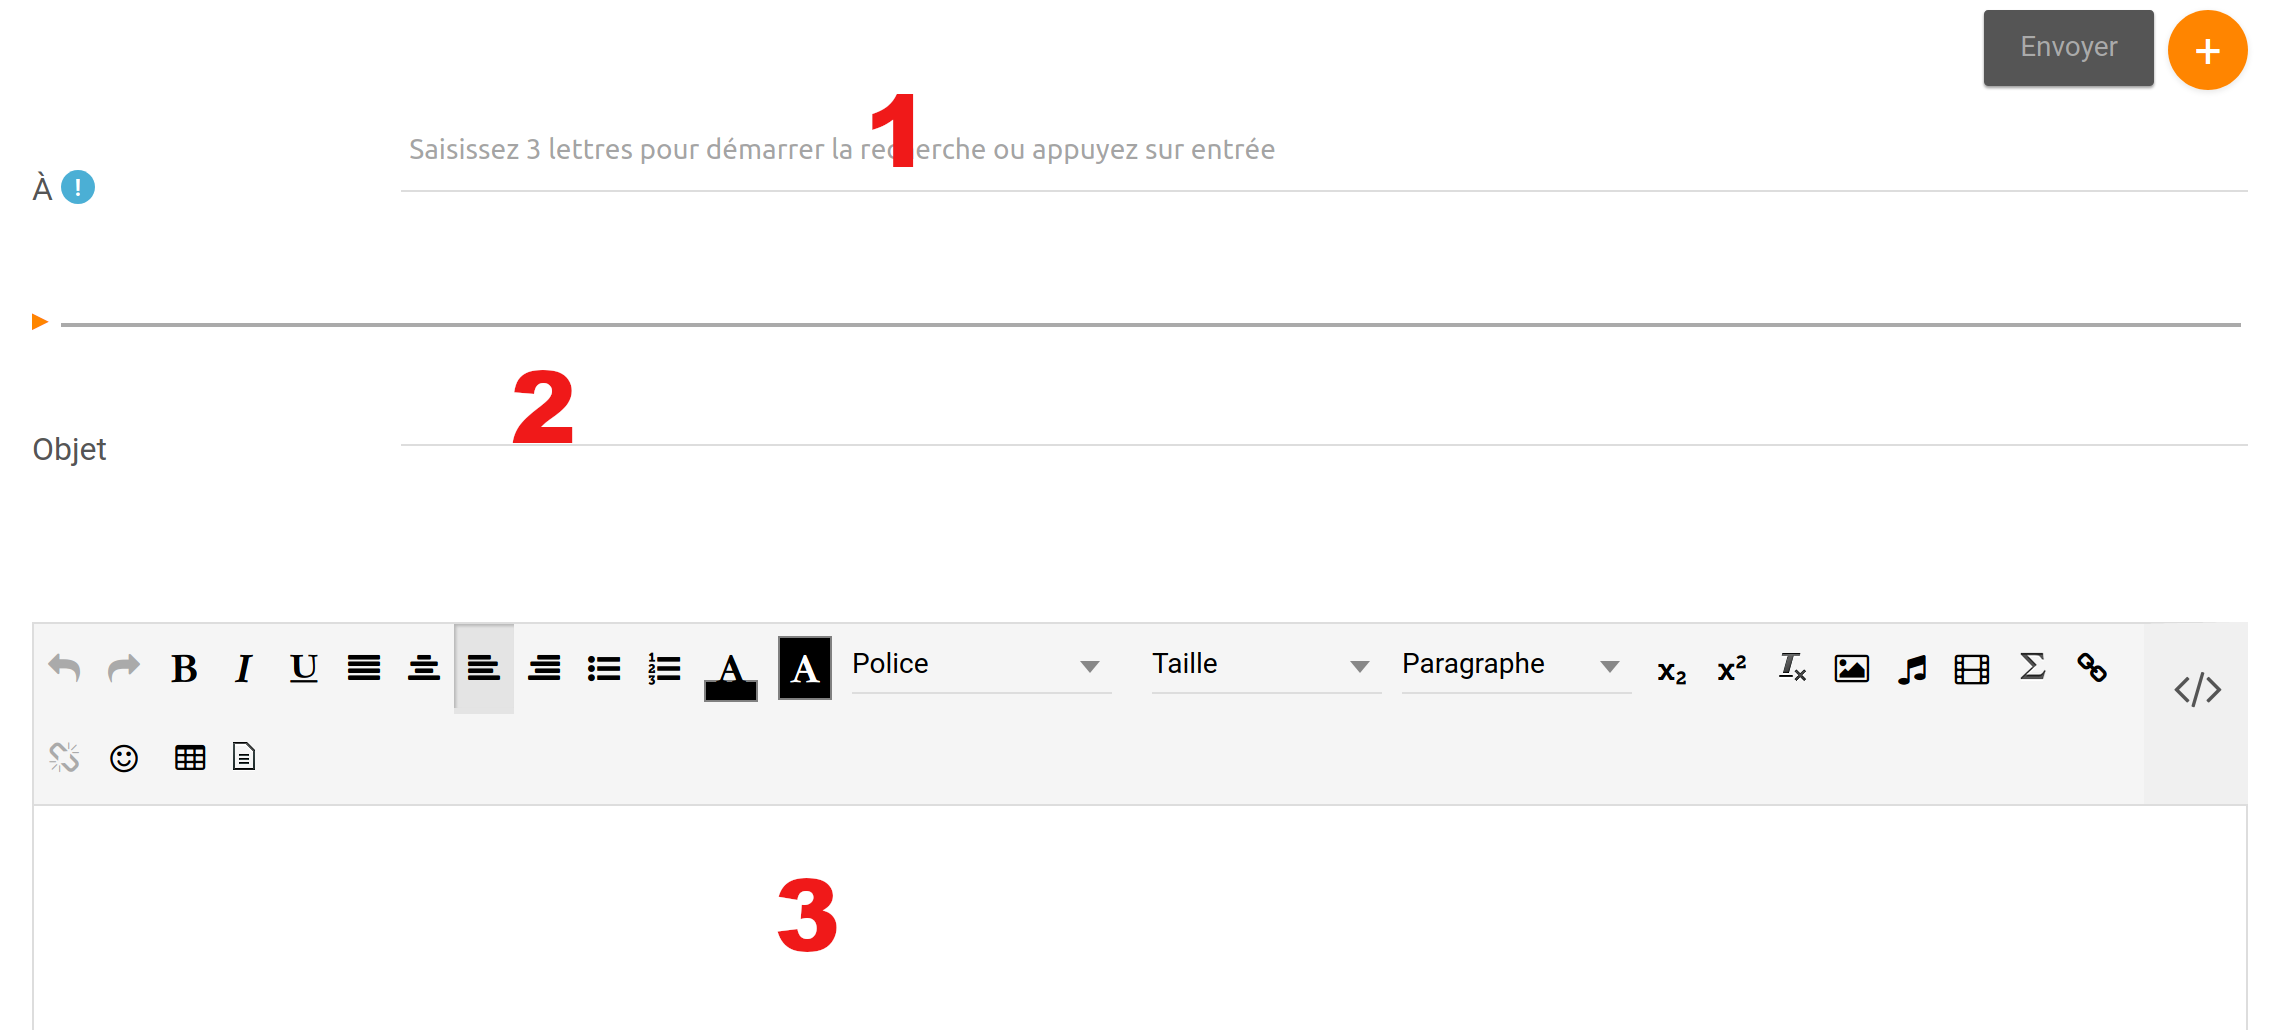
\includegraphics[width=6cm]{ressources/ecriremail.png}
        \end{center}
        \begin{enumerate}
            \item \emph{adresse mail} ou nom de la personne destinataire (les adresses des élèves ou enseignants présents sur le lycée connecté sont pré-enregistrées),
            \item \emph{objet} ou titre du mail,
            \item \emph{corps} ou contenu.
        \end{enumerate}
    \end{enumerate}
    \end{activite}

\end{frame}
\subsection{Casier}
\begin{frame}
    \frametitle{Casier}

Il existe de nombreuses applications utiles pour travailler ou communiquer.
\begin{activite}
\begin{enumerate}
    \item Cliquer sur l'icône \textbf{Mes applis}:
    \begin{center}
    \centering
    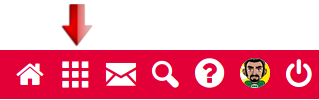
\includegraphics[width=5cm]{ressources/bandeauapp.png}
    \end{center} 
    \item Cliquer sur l'icône \emph{Casier}:
    \begin{center}
    \centering
    
\includegraphics[width=1cm]{ressources/casier.png}
    \end{center}
    \item Cliquer sur \emph{Déposer dans un casier}.
    \item Déposer un document (image, texte\dots) dans le casier de \emph{Christophe Viroulaud}.
\end{enumerate}
\end{activite}

\end{frame}
\subsection{Évaluation automatisée}
\begin{frame}
    \frametitle{}

    \begin{activite}
        \begin{enumerate}
            \item Cliquer sur l'icône \emph{Exercices}:
            \begin{center}
            \centering
            
\includegraphics[width=1cm]{ressources/exercices.png}
            \end{center}
            \item Réaliser l'évaluation \textbf{entraînement rentrée}.
            \item Ne pas oublier d'envoyer les résultats en fin d'évaluation.
        \end{enumerate}
        \end{activite}

\end{frame}
\section{Outils divers}
\subsection{Espace personnel}
\begin{frame}
    \frametitle{Espace personnel}

Chaque élève possède un disque dur personnel accessible depuis n'importe quel poste de l'établissement.
\begin{activite}
\begin{enumerate}
    \item Depuis le bureau (écran principal à l'ouverture de l'ordinateur) cliquer sur \emph{Poste de travail}
    \begin{center}
    \centering
    
\includegraphics[width=1cm]{ressources/poste.png}
    \captionof{figure}{L'icône peut être légèrement différente selon le poste.}
    \end{center}
    \item Repérer les disques \emph{personnel} et \emph{groupes}.
    \item Dans le disque \emph{personnel} créer un dossier \textbf{SNT}.
\end{enumerate}
\end{activite}

\end{frame}
\subsection{Dossier compressé}
\begin{frame}
    \frametitle{Dossier compressé}

    Pour envoyer  (par mail, messagerie\dots) un ensemble de fichiers en une fois on utilise un \emph{dossier compressé}. On parle également de dossier \emph{zip}.
    \begin{center}
    \centering
    
\includegraphics[width=1cm]{ressources/zip.png}
    \captionof{figure}{L'icône peut varier selon les postes.}
    \label{IMG}
    \end{center}

\end{frame}
\begin{frame}
    \frametitle{}

    \begin{activite}
    \begin{enumerate}
        \item Sur le site \url{https://cviroulaud.github.io}, télécharger le dossier \emph{entrainement\_dossier.zip}
        \item Retrouver le dossier compressé dans le dossier \emph{Téléchargements} de l'ordinateur ou l'ouvrir directement à la fin du téléchargement.
        
        
    \end{enumerate}
    \end{activite}
    \begin{aretenir}[]
        À cette étape les fichiers sont visibles mais ne sont pas extraits du dossier compressé. Il faut exécuter les points suivants pour terminer le processus d'extraction.
        \end{aretenir}
\end{frame}
\begin{frame}
    \frametitle{}
\setcounter{compteuractivite}{8}
    \begin{activite}
    \begin{enumerate}
        \setcounter{enumi}{2}
        \item Sélectionner tous les fichiers présents dans le dossier.
        \item Cliquer sur le bouton \textbf{Extraire}.
        \begin{center}
        \centering
        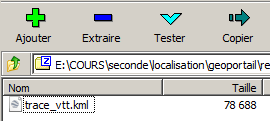
\includegraphics[width=3cm]{ressources/extraire.PNG}
        \end{center}
        \item Cliquer sur le bouton de sélection d'emplacement et choisir le dossier \textbf{SNT}.
        \begin{center}
        \centering
        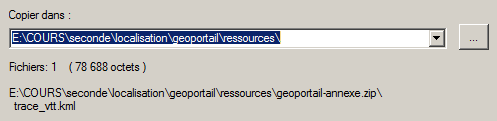
\includegraphics[width=5cm]{ressources/extraire2.PNG}
        \captionof{figure}{Cliquer sur les 3 points à droite.}
        \label{IMG}
        \end{center}
        \item Valider pour extraire.
        \item Depuis le \emph{Poste de travail}, retrouver le fichier extrait dans le dossier \textbf{SNT}.
    \end{enumerate}
    \end{activite}

\end{frame}
\end{document}